%----------------------------------------------------------------------------------------------------------------------------------------------------------%
\chapter{Theoretical context}
%----------------------------------------------------------------------------------------------------------------------------------------------------------%
\epigraph{Each source that I read, I would look through the bibliography and the footnotes, and use that as a map for the next thing I would read.}{\textit{Alexander Chee}}
%----------------------------------------------------------------------------------------------------------------------------------------------------------%
\section{Bacteria and bacterial infections}
\paragraph{Bacteria} are prokaryotic organisms, generally single-celled, which are part of the Monera animal kingdom. Their sizes range from between \SI{30}{\micro\metre} and \SI{100}{\micro\metre} and are ubiquitous\footnote{Ubiquitous: found everywhere} organisms. This form of life is believed to be the first one to have ever appeared on Earth, as well as the one responsible for the oxygen-rich atmosphere the Earth currently has. Some species are hard to culture in a laboratory environment, but generally, those that can be cultured in a controlled environment are grown in agar plates\cite{murrayMicrobiologiaMedica2013}. \newline
\paragraph{Agar} is used as a base medium to grow bacteria due to the fact that it is indigestible for the majority of bacteria, while keeping them humid. Together with growth mediums, such as Lysogeny Broth, bacteria thrive in this environment, allowing them to proliferate and create colonies, which can be observed without the need of optic magnifying equipment. Sometimes, together with the growth medium, additives such as mannitol or salt are added. These are used to improve or impede bacterial growth, modify their conditions, so they develop differently or as an identification tool. For this research MSA (mannitol-salt agar) was used, since \emph{Staphylococcus aureus} ferments the mannitol, producing acid, which in turn decolorizes the plate's integrated pH indicator from red to yellow, whilst the salt prevents the growth of bacteria that are not of interest to the study (since \emph{Staphylococci} are able to sustain high levels of salt concentrations)\cite{gamazoManualPracticoMicrobiologia2010}.
\paragraph{Pathogenic bacteria} are bacteria that have the ability to cause disease\footnote{A disease is a particular abnormal condition that negatively affects the structure or function of all or part of an organism, and that is not immediately due to any external injury\cite{DorlandsMedicalDictionary2010}.} These are not the most common type of bacteria, as the majority of them are either harmless or beneficial to the human body through symbiosis, such as the bacteria that help with digestion in the stomach\cite{murrayMicrobiologiaMedica2013}.
%----------------------------------------------------------------------------------------------------------------------------------------------------------%
\section{The enemy: \emph{Staphylococcus aureus}}
\paragraph{}\emph{Staphylococcus aureus} (also known as Staph) is a GRAM-positive bacteria, the most studied and one of the most prevalent\footnote{Prevalence: the percentage of a population that is affected with a disease}of its genus. Staph bacteria are usually harmless. However, they can, in some cases, cause serious infections that, in some cases, can lead to sepsis or death. Some of its distinctive characteristics include having a very thick glycopeptide wall, which allows it to withstand extreme temperatures and osmotic pressures, therefore rendering most classic methods of food conservation (such as cooking, smoking, freezing, or salting) completely useless against said bacteria; a protein A capsid, which binds to many eukaryote organisms; as well as thermoresistant enterotoxins. It's an extremely resistant (and thus ubiquitous) bacteria. It can be found in human skin, especially below the nails, and mucotic surfaces (such as the mouth or the nose), as well as in certain foods such as ham (even after it's been cooked or curated), eggs, poultry and both raw and cooked dough.\newpage
\begin{wrapfigure}{r}{0.5\textwidth}\begin{center}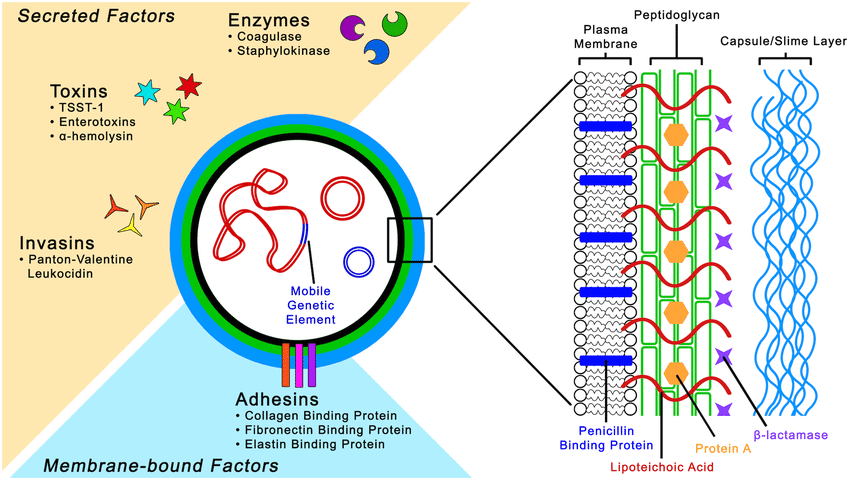
\includegraphics[width=0.48\textwidth]{staph_parts.png}\end{center}\caption{Parts of \emph{Staphylococcus aureus}\cite{kongCommunityAssociatedMethicillinResistantStaphylococcus2016}.}\end{wrapfigure}\paragraph{}Staphylococcus aureus has three main parts to its virulence: its cell wall, its membrane-bound factors and its secreted factors. Staph's \textbf{cell wall} is made up of three parts, going from inside to the outside of the cell: a plasma membrane, a peptidoglycan layer and a slime (sometimes also called capsule) layer\cite{kongCommunityAssociatedMethicillinResistantStaphylococcus2016}. %source: %
The plasma membrane consists of a lipid bi-layer that is semipermeable\footnote{Semipermeable: it lets water and ions through, but not other molecules. This transport will always be in favour of the pressure gradient, which means that it cannot insert any kind of substance into an environment that has a higher pressure than the other side}, which regulates the transport of materials entering and exiting the cell. Integrated inside them are a type of integral protein\footnote{Integral protein: protein that is situated perpendicularly to the cell wall, allowing for communication between the exterior and interior} called penicillin-binding protein (PBP), amongst other  proteins such as protein channels. We will only talk about PBPs because they are the Achilles's Heel of bacteria, as long as one has the proper tools to exploit it. Whilst the name implies PBPs are only sensible to penicillin, the name actually came to be this way because it's how they were discovered, and in fact could be resistant to it but sensible to other similar antibiotic agents. Variations in this protein may lead in some cases to antibiotic resistance, such as MRSA (\emph{Methicillin-Resistant \emph{Staphylococcus aureus}}), a variation of Staph that is the result of a variation in this protein called PBP2A. The different variations of \emph{Staphylococcus aureus} will be discussed in more detail in a following section. \newline
\emph{Staphylococcus aureus}, like all other members of the \emph{Staphylococcus} family, have very thick peptidoglycan layers. This grants them protection from extreme temperatures and high osmotic pressures, which means these bacteria can colonize cooked food and food that has been salted. The most notable example is ham, either cooked, smoked or cured. Since little to no other bacteria can survive in those conditions, \emph{Staphylococcus aureus} takes advantage of it and starts reproducing, draining the resources available for other bacteria.
%----------------------------------------------------------------------------------------------------------------------------------------------------------%
\section{The enemy's attacks}
\paragraph{}\emph{Staphylococcus aureus} is a species that can cause a handful of different diseases, ranging from, most frequently, skin and respiratory tract infections to infective endocarditis, toxic shock syndrome or osteomyelitis. Several variations of this pathogen exist, with increasing levels of antibiotic resistance: MSSA (\emph{Methicillin-Sensitive Staphylococcus aureus}), having no resistance; MRSA (\emph{Methicillin-Resistant Staphylococcus aureus}); and VRSA (\emph{Vancomycin-Resistant Staphylococcus aureus}), the   latter for which no antibiotic concoction that can eradicate the infection is known, and the patients have to use experimental treatments. VISA (\emph{Vancomycin-intermediate Staphylococcus aureus}) is a variation that has medium resistance to vancomycin, being an intermediate step between MRSA and VRSA. VISA and VRSA are what we would call a superbug, a microbe that has developed resistance to more quantity of antibiotic than is safe to consume. Studies have discovered that this genetic factor has been developed by different lineages separately, indicating that there is not a common ancestor of MRSA strains. This case is the bacteria equivalent of carcinization \footnote{Carcinization: the discovery that several species have evolved into crabs} or tree leaves\footnote{Tree leaves were developed independently by several species at the same time, in completely different parts of the world.}
\paragraph{}One of Staph's most notorious abilities is using the body's own proteins to disguise itself and thus avoid detection and phagocytosis by the host's immune system. It accomplishes this task by using enzymes called coagulases, which enable the transformation of fibrinogen \footnote{A glycoproteic complex produced in the liver and present in the blood of all vertebrates.} to fibrin \footnote{fibrinogen after being stimulated by either thrombin or \emph{staphylothrombin}, the result of a molecular pathway stimulated by coagulase. It helps in clotting the blood in the event of vascular or tissue injury such as a cut or bruise. }\cite{murrayMicrobiologiaMedica2013}. Only 11 other \emph{Staphylococcus} family members are coagulase-positive. To test for this enzyme in the laboratory there are two main methods which are usually combined: culture of the sample on a Baird-Parker agar medium, a selective and differential medium which contains lithium chloride and tellurite as to inhibit the growth of other microbes; while also including pyruvate and glycine, which promote the growth of \emph{Staphylococci} colonies, showing in colour black and with an opaque zone around the colony. This opaque zone represents the effect of the coagulase. Another way to test for coagulase is to perform a coagulase test. This test generally requires a small quantity (generally 2 mL) of sheep blood serum, which will gelatinize if coagulase is present.
\paragraph{}\emph{Staphylococcus aureus} contains an important quantity of \textbf{toxins}, compounds that grant \emph{Staph} most of its pathogenicity. Many of its virulence factors can be described as such. Toxins are usually defined as poisonous substances, which, in our case, means that they have the capacity to mess with the host body directly, without need of a mediating entity. This category doesn't include, for example, those molecules intended to combat the host's defence mechanisms or scavenge reactive oxygen. We'll also exclude those situated on its membrane for the purpose of cell binding. Staph has several kinds of toxin in its arsenal: membrane-damaging toxins (which can be receptor-mediated or not), receptor-interfering toxins (not membrane-damaging), enzymes, and pathway blockers.\newline
\begin{itemize}
\item[$\bullet$] Membrane-damaging toxins. Several of \emph{Staphylococcus aureus}' toxins target the cytoplasmic membrane of the host's cells. These lead to pore formation in it, which provokes the outflux of vital molecules of the cell which, in turn, leads to cytolysis\footnote{Cytolysis: Cell bursting due to osmotic pressure imbalance between the inside and the outside of it}.
   \begin{itemize}
        \item Receptor-mediated. Many of the cytolytic toxins of \emph{Staphylococcus aureus} have been shown to require receptor interaction for their lytic activity. The best-known toxin of this kind is Alpha-toxin, also known as Alpha-hemolysin, which is its major cytotoxic agent, and is lytic to red blood cells and certain leukocytes, but not to neutrophils. Whilst at low concentrations it has been shown to be dependent on the interaction with cells' ADAM10 receptors, in higher concentrations of this toxin, this interaction is no longer necessary. Other toxins of this type include  PVL (Panton-Valentine Leucocidin) and Gamma-toxin.
        \item Non-receptor-mediated. In 2007, a toxin family that includes the Delta-toxin called the Phenol-Soluble Modulins (PSMs) was discovered. PSMs trigger an inflammatory response by interacting with the FPR2 receptor, however they can carry cytolytic activity independently of said interaction. Delta-toxin has been linked to allergic skin disease and atopic dermatitis by degrading mast cells\footnote{Mast cell: immune cell specific for connective tissue}. This kind of toxin contributes to neutrophil lysis after phagocytosis\footnote{Phagocytosis is a process done by neutrophils in which the neutrophil consumes the foreign agent}, which might partly explain why the development of \emph{Staphylococcus aureus} vaccines that work by enhancing a type of phagocytosis have failed so far.
   \end{itemize}
\item[$\bullet$] Receptor-function-interfering toxins. The toxins that fall into this category are enterotoxins\footnote{Enterotoxins are those toxins that target the intestines.} These typically cause vomit and diarrhoea. \emph{S. aureus} strains can produce a wide array (around 20) of entero and entero-like toxins. The most famous \emph{Aureus} super-antigen\footnote{Super-antigen: type of antigens that results in excessive activation by the immune system}, the 22-kD toxic shock syndrome toxin (TSST), belongs to this group. TSS is a very severe and potentially fatal disease. \emph{Staphylococcus aureus} also secretes a series of proteins that interfere with leukocyte receptors to evade recognition and thus activation of the immune system. CHIPS (Chemotaxis Inhibitory Protein of \emph{Staphylococcus aureus}), which binds to the C5aR and FPR receptors, impairs the recognition of bacterial formylated peptides by the FPR receiver and blocks the activation of leukocytes via C5aR. \emph{S. aureus} also has other proteins that work similarly to these, such as FLIPr.
\item[$\bullet$] Enzymes. Many enzymes secreted by \emph{Staphylococcus aureus} either degrade host molecules or interfere with its metabolic or signalling cascades. A few of them are proteases, which some non-specific ones have the ability to degrade host proteins in a broad proteins, leading to tissue destruction and necrosis, but may also have some more specific effects, for example the destruction of insulin B. Its two coagulases (staphylocoagulase and Willebrand factor) fall into this category.
\end{itemize}
%----------------------------------------------------------------------------------------------------------------------------------------------------------%
\section{Our weapons}
\paragraph{} The tools we have at our disposal to fight off this infection fall into two main categories: chemical factors and biological factors.
\paragraph{} The chemical factors are drugs, and they depend both in quantity and type on the variation a particular case falls in. It is \textbf{extremely important} to find out the level of antibiotic resistance that a specific infection has before administering any antibiotic, as this treatment course will cause side effects such as killing gut bacteria, diminishing defence system capabilities, and increasing the possibility to develop yet more resistant infections. Generally, a large-spectrum antibiotic has an adequate risk-to-benefits ratio of causing the previously mentioned side effects, so they may be used before switching to a more specific (and in some cases even more violent) treatment.
\paragraph{}\begin{wrapfigure}{r}{0.35\textwidth}\begin{center}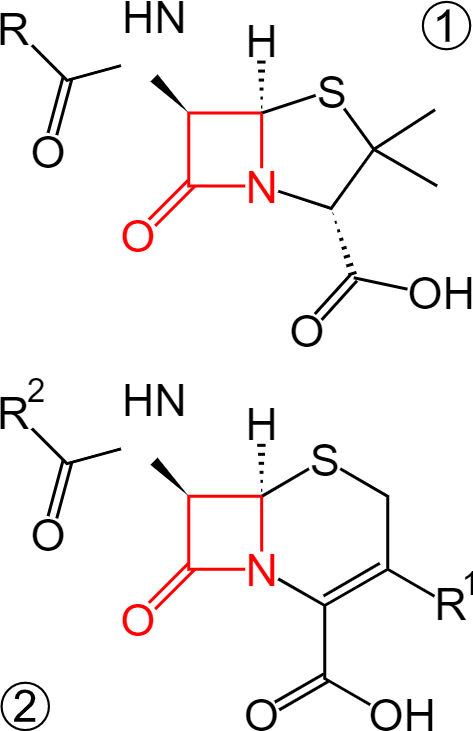
\includegraphics[width=0.30\textwidth]{assets/beta-lactam.png}\end{center}\caption{Organic chemistry structure of penicillin (top) and cephalosporin (bottom). \beta-lactam ring in red. Source: WikiMedia}\vspace{-0.30\linewidth}\end{wrapfigure}Starting with the treatment to the least resistant strains of \emph{Staphylococcus aureus}, a \beta-lactam antibiotic (such as methicillin, oxacillin, cloxacillin and penicillin) is the weapon of choice to fight against an MSSA infection. This is because this specific chemical part (just a \beta-lactam ring does nothing by itself) has the ability to inhibit cell wall biosynthesis on the bacterial intruder's body. But once the \beta-lactam ring is cut by an enzyme secreted by the bacteria itself, this type of antibiotic suddenly loses effect against them.
\paragraph{}That's where vancomycin comes in. It is a type of glycopeptide antibiotic, just like \beta-lactam, and works by blocking the construction of a cell wall, as all of its type do. This treatment is very invasive and only indicated for the treatment of extremely serious, life-threatening infections by Gram-positive bacteria that have shown to be unresponsive to other antibiotics.\begin{wrapfigure}{l}{0.35\textwidth}\begin{center}
\includegraphics[width=0.30\textwidth]{assets/vancomycin.png}\end{center}\caption{Organic chemistry structure of vancomycin. Source: WikiMedia}\vspace{0.15\linewidth}\end{wrapfigure}\newline It can be taken as a pill or as an injectable fluid, the latter form proving to be much more effective than the former. This treatment is incompatible with aminoglycosides, a type of antibiotic that inhibit protein synthesis, as it can lead to nephrotoxicity\footnote{Nephrotoxicity: damage to the kidneys} and ototoxicity\footnote{Ototoxicity: damage to hearing}. Vancomycin can induce platelet-reactive antibodies in the patient, leading to internal bleeding, with petechial haemorrhages on the tongue and bruises on most of the body. Unfortunately, even with use of vancomycin, \emph{Staphylococcus aureus} can develop resistance. In this case, no other option than using a biological factor is left. There has been one study in 2020 that discovered that by modifying the bacteria with a cationic oligo peptide\footnote{Cationic oligo peptide: sequence of two or more amino acids that is positively charged}, vancomycin resistance could be bypassed. This could be a good solution temporarily as we wait for phage therapy to get improved on and approved, if it was a sufficiently studied option, which is not. This was discovered in 2020, while bacteriophage trials have been ongoing since the mid 2000s.
\paragraph{}The biological factor is a bacteriophage, called P68. It comes from the \emph{Caudovirales} order, which means that it is a bacteriophage with tail.  This treatment is still in testing, but it appears to be effective and lead to low adverse results. If possible, it would be preferable to use bacteriophage therapy (shortened to phage therapy) instead of going for antibiotics, as it can lead to less side effects than antibiotics, as it only attacks specific bacteria. This means, unfortunately, that the infection has to be pinpointed with extreme accuracy. The use of this treatment also negates the risk of bacteria developing antibiotic resistance. It is, however, unclear whether the bacteriophage could mutate into a dangerous strain. This class of vira has been studied since the late 19th century after being discovered by accident in water from a river in India. This research, however, was dropped due to penicillin being discovered and used, sometimes abusively, as the main purpose of this research was to use it on war casualties in order to reduce mortality caused by infections.
\newpage{}\begin{wrapfigure}{r}{0.35\textwidth}\begin{center}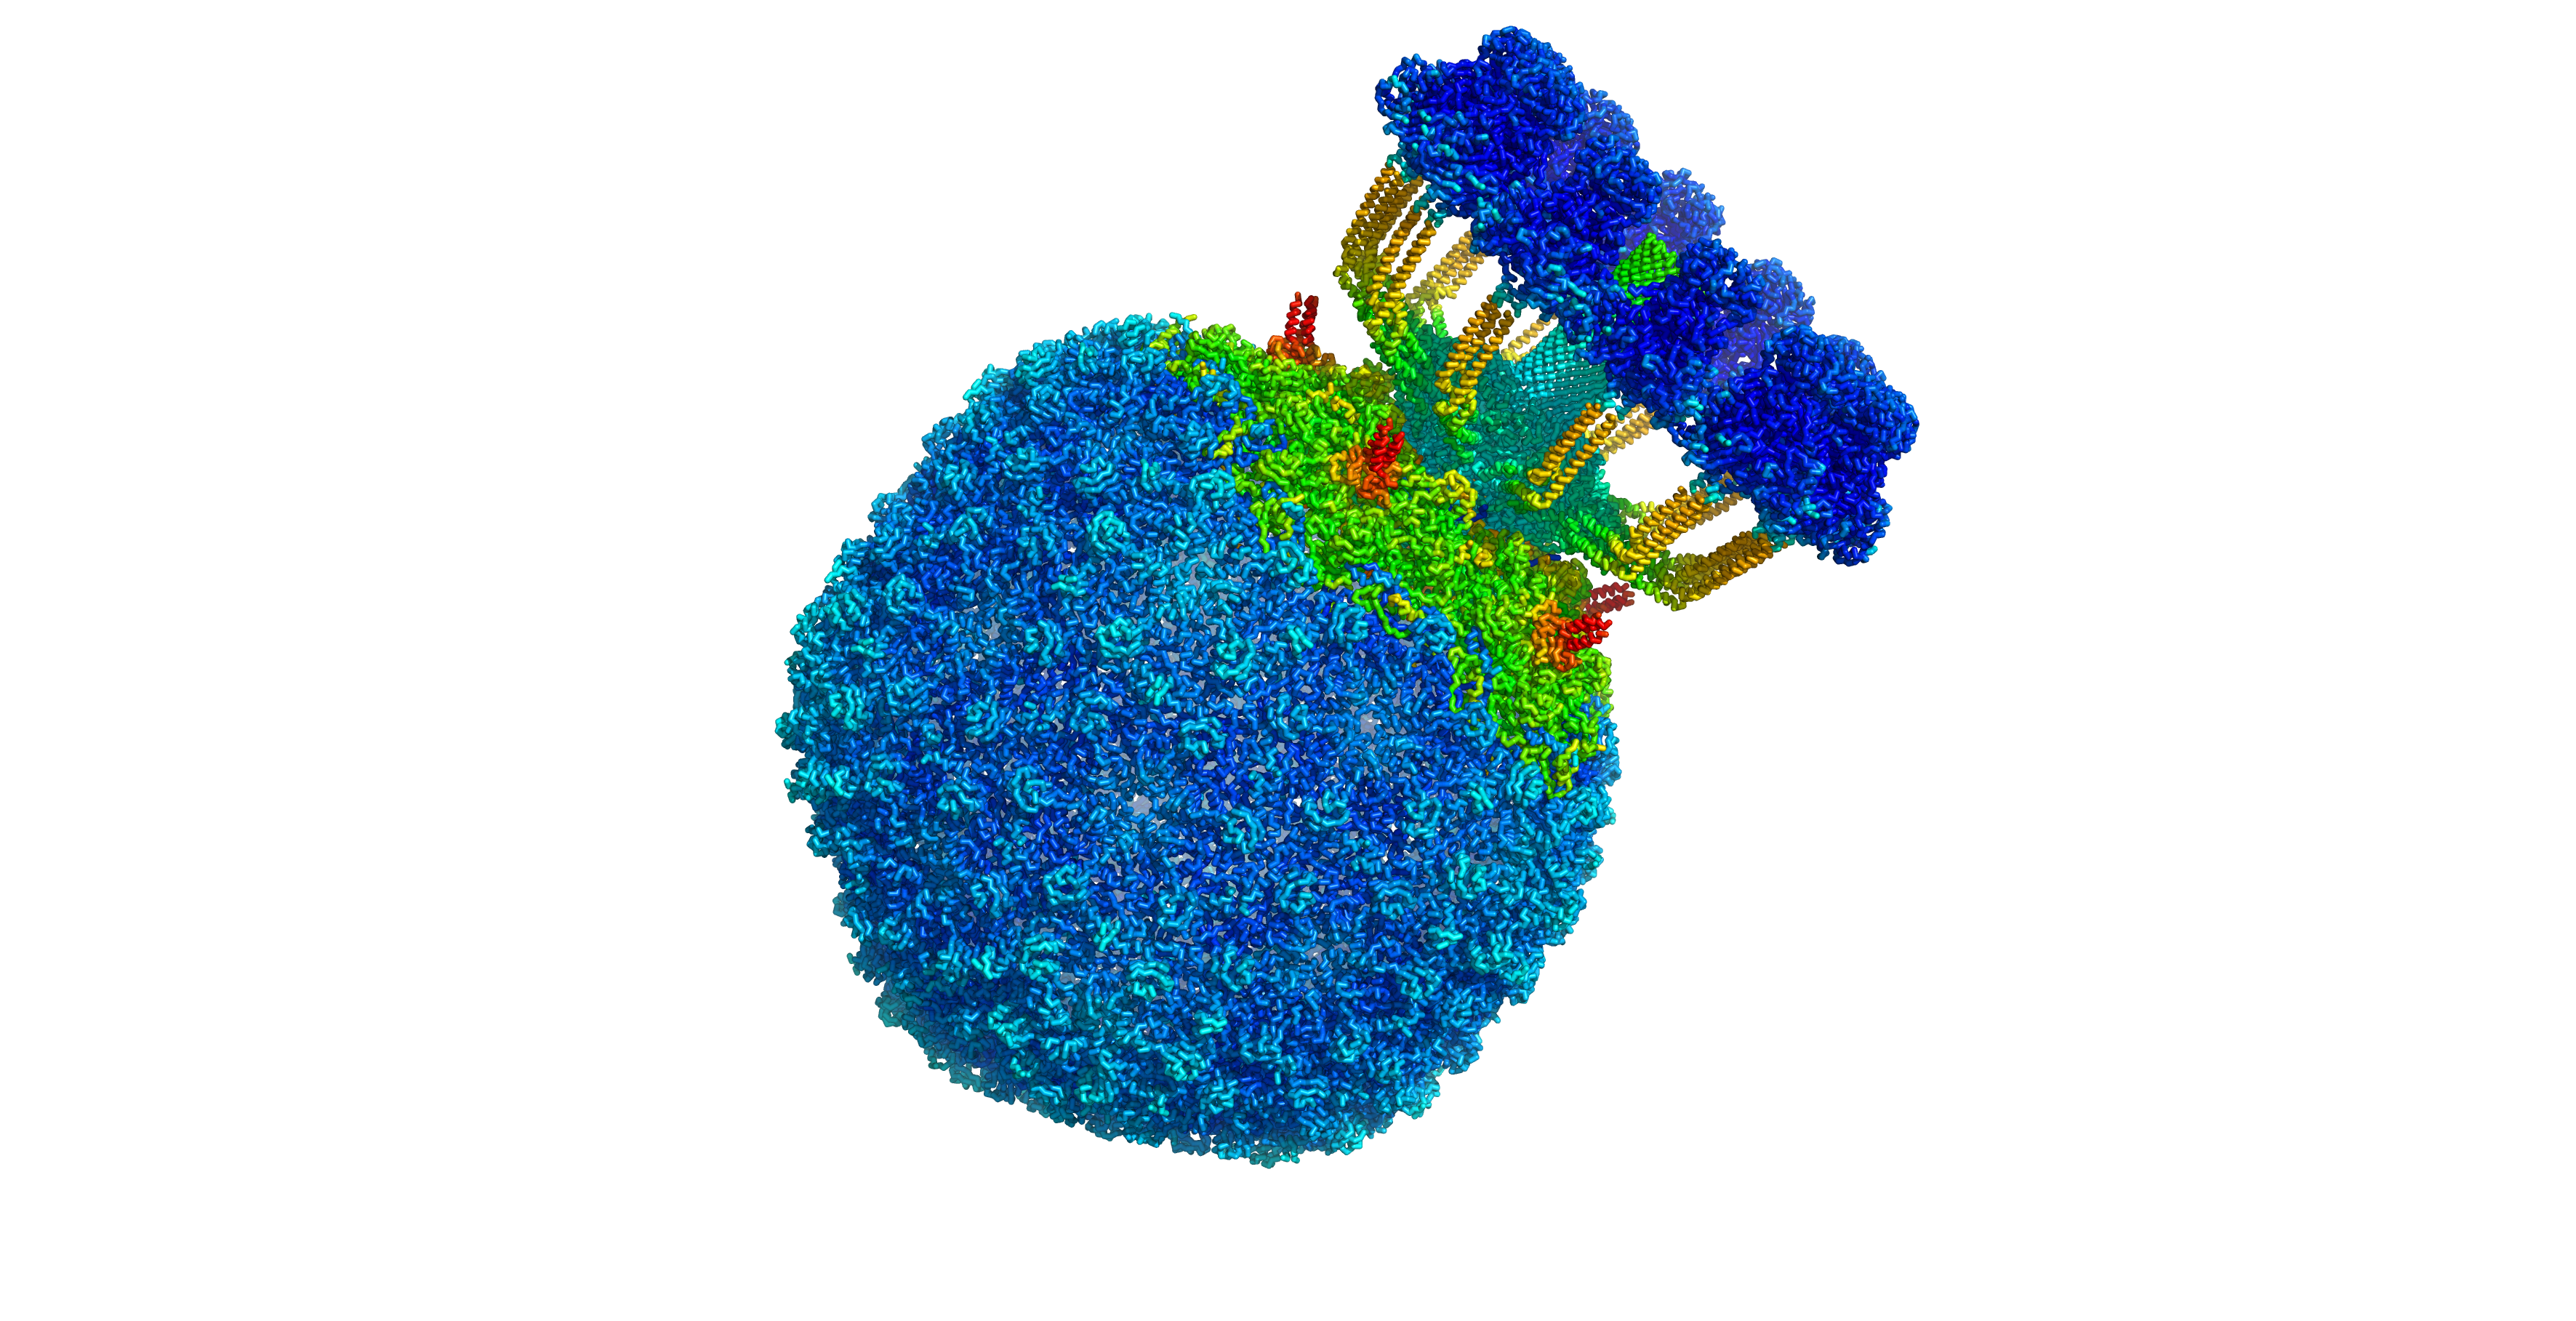
\includegraphics[width=0.30\textwidth]{assets/staph_side.png}\end{center}\caption{P68 structure. Source: Own results}\end{wrapfigure}Bacteriophages work in an interesting manner. They work by detecting one very specific bacteria, just like any other virus does with the type of cell they evolved for, then bind to it and inject their genetic material, which then in turn the bacteria considers as its own, inserts it into its own genetic sequence and starts producing the proteins the virus requires, but it doesn't eject them. Once the bacteria is full of phages, a special lytic compound is released which bursts the cell membrane in such a way that it resembles an explosion, but instead of heating up everything in a radius, spreads millions more of bacteriophages, which then bind to other bacteria and the cycle repeats until there's no more bacteria left. The fight from the bacteria point of view consists mostly on trying to outnumber and outreproduce the phages in order to have a chance of survival, even if minimal. There is no known bacteria that shows resistance to phages. That is probably because, unlike the chemical factors, phages can evolve and improve with each generation.
